\chapter{Results\label{cha:results}}

In the following chapter, the achieved results of the concept are presented. The described approaches are evaluated with regards to the common metrics precision, recall, and F1-Score. Different hyperparameter setups are discussed and visualised in graphs. In particular, the language models Bert, XL-Transformers and GPT-2 as described in \ref{transformer-approach} are compared. Additionally, the regression-based method as described in \ref{sec:regression} and the multi-classification method as described in \ref{sec:classification} are compared, showing advantages or disadvantages among each other.


\section{Experimental Setup}
\subsection{Anomaly Detection on one Dataset \label{sec:ad_one_ds_result}}
For evaluating the model, the OpenStack datasets "normal log dataset 2" (referenced to as original dataset from now on) containing 137k log lines and the "log dataset having performance anomalies" containing 18k log lines (referenced to as test dataset from now on), provided by the DeepLog authors at the University of Utah are used \cite{utah_dataset}. The original dataset stems from logs from running multiple OpenStack instances for 20 hours and 13 minutes for the original dataset and 2 hours and 17 minutes for the test dataset on CloudLab \cite{cloudlab}. Since the test dataset contains anomalies which are only detectable by inspecting the parameters of the log events, as described in \ref{fig:parsing}, i.e. the variable part of the log event which is not visible in the template after parsing, anomalies are injected into the dataset, yielding a labeled dataset for testing. This is necessary due to the assumptions specified in \ref{sec:requirements_and_assumptions}.
In order to assess the quality of the used word embeddings, log alterations are additionally injected into the dataset containing anomalies, in order to simulate the instability of logs as described in \ref{sec:logs_alteration}.
\subsection{Transfer Learning}
In order to examine the ability of the model to transfer the knowledge obtained from one dataset to a different one, the same OpenStack log dataset as utilised in \ref{sec:ad_one_ds_result} is used as a basis. Then, in order to simulate a different dataset, various of the alterations discussed in \ref{sec:logs_alteration} are injected all at once. For the following experiments, line shuffling, duplication and deletion, and word insertion, removal and replacement are injected into the dataset at various ratios.


\section{Evaluation}
\subsection{String cleansing}
String cleansing, as described in \ref{sec:template_cleansing}, can potentially  improve distinguishability between templates drastically in the used dataset.
For Bert, the pairwise cosine distances before cleansing are depicted in figure \ref{fig:bert_before_cleansing}, after cleansing in figure \ref{fig:bert_after_cleansing}. The corresponding templates to the indices on the x and y axes before and after cleansing can be found in table \ref{tab:templates_before_cleansing} and table \ref{tab:templates_after_cleansing} respectively.
The cosine distances before and after cleansing for GPT-2 can be found in figure \ref{fig:gpt_before_cleansing} and figure \ref{fig:gpt_after_cleansing}, and for XL-Transformer in figure \ref{fig:xl_before_cleansing} and figure \ref{fig:xl_after_cleansing}, respectively. The average pairwise cosine distances between templates before and after cleansing can be seen in table \ref{tab:average_pairwise_cos_distances}.
Note that the cosine distances between templates appear to be relatively low for GPT-2 before and after cleansing. Even though cleansing results in a two-fold increase in the distances, the initial value is already very low. We can see how the distinguishability between templates increases for Bert and even more impressively for XL-Transformers. While Bert has a slightly higher average pairwise cosine distance before cleansing, XL-Transformers highly benefits from cleansing with an average value of 0.62. This underlines the importance of this step in order to meet the requirements postulated in \ref{sec:word_vectorization}, depending on the deployed language models.



\begin{table}[ht]
\centering
\begin{small}
\begin{tabular}{ p{1.3cm} p{2.5cm} p{2.5cm} }
\toprule
Model & Before cleansing & After cleansing\\
\midrule
XL & 0.2232 & 0.6223\\
Bert & 0.2416 & 0.4449\\
GPT-2 & 0.0024 & 0.0047 \\ 

\bottomrule
\end{tabular}
\caption{Average pairwise template cosine distances.}
\label{tab:average_pairwise_cos_distances}
\end{small}
\end{table}


\begin{figure}[!tbp]
  \centering
  \subfloat[Before cleansing.]{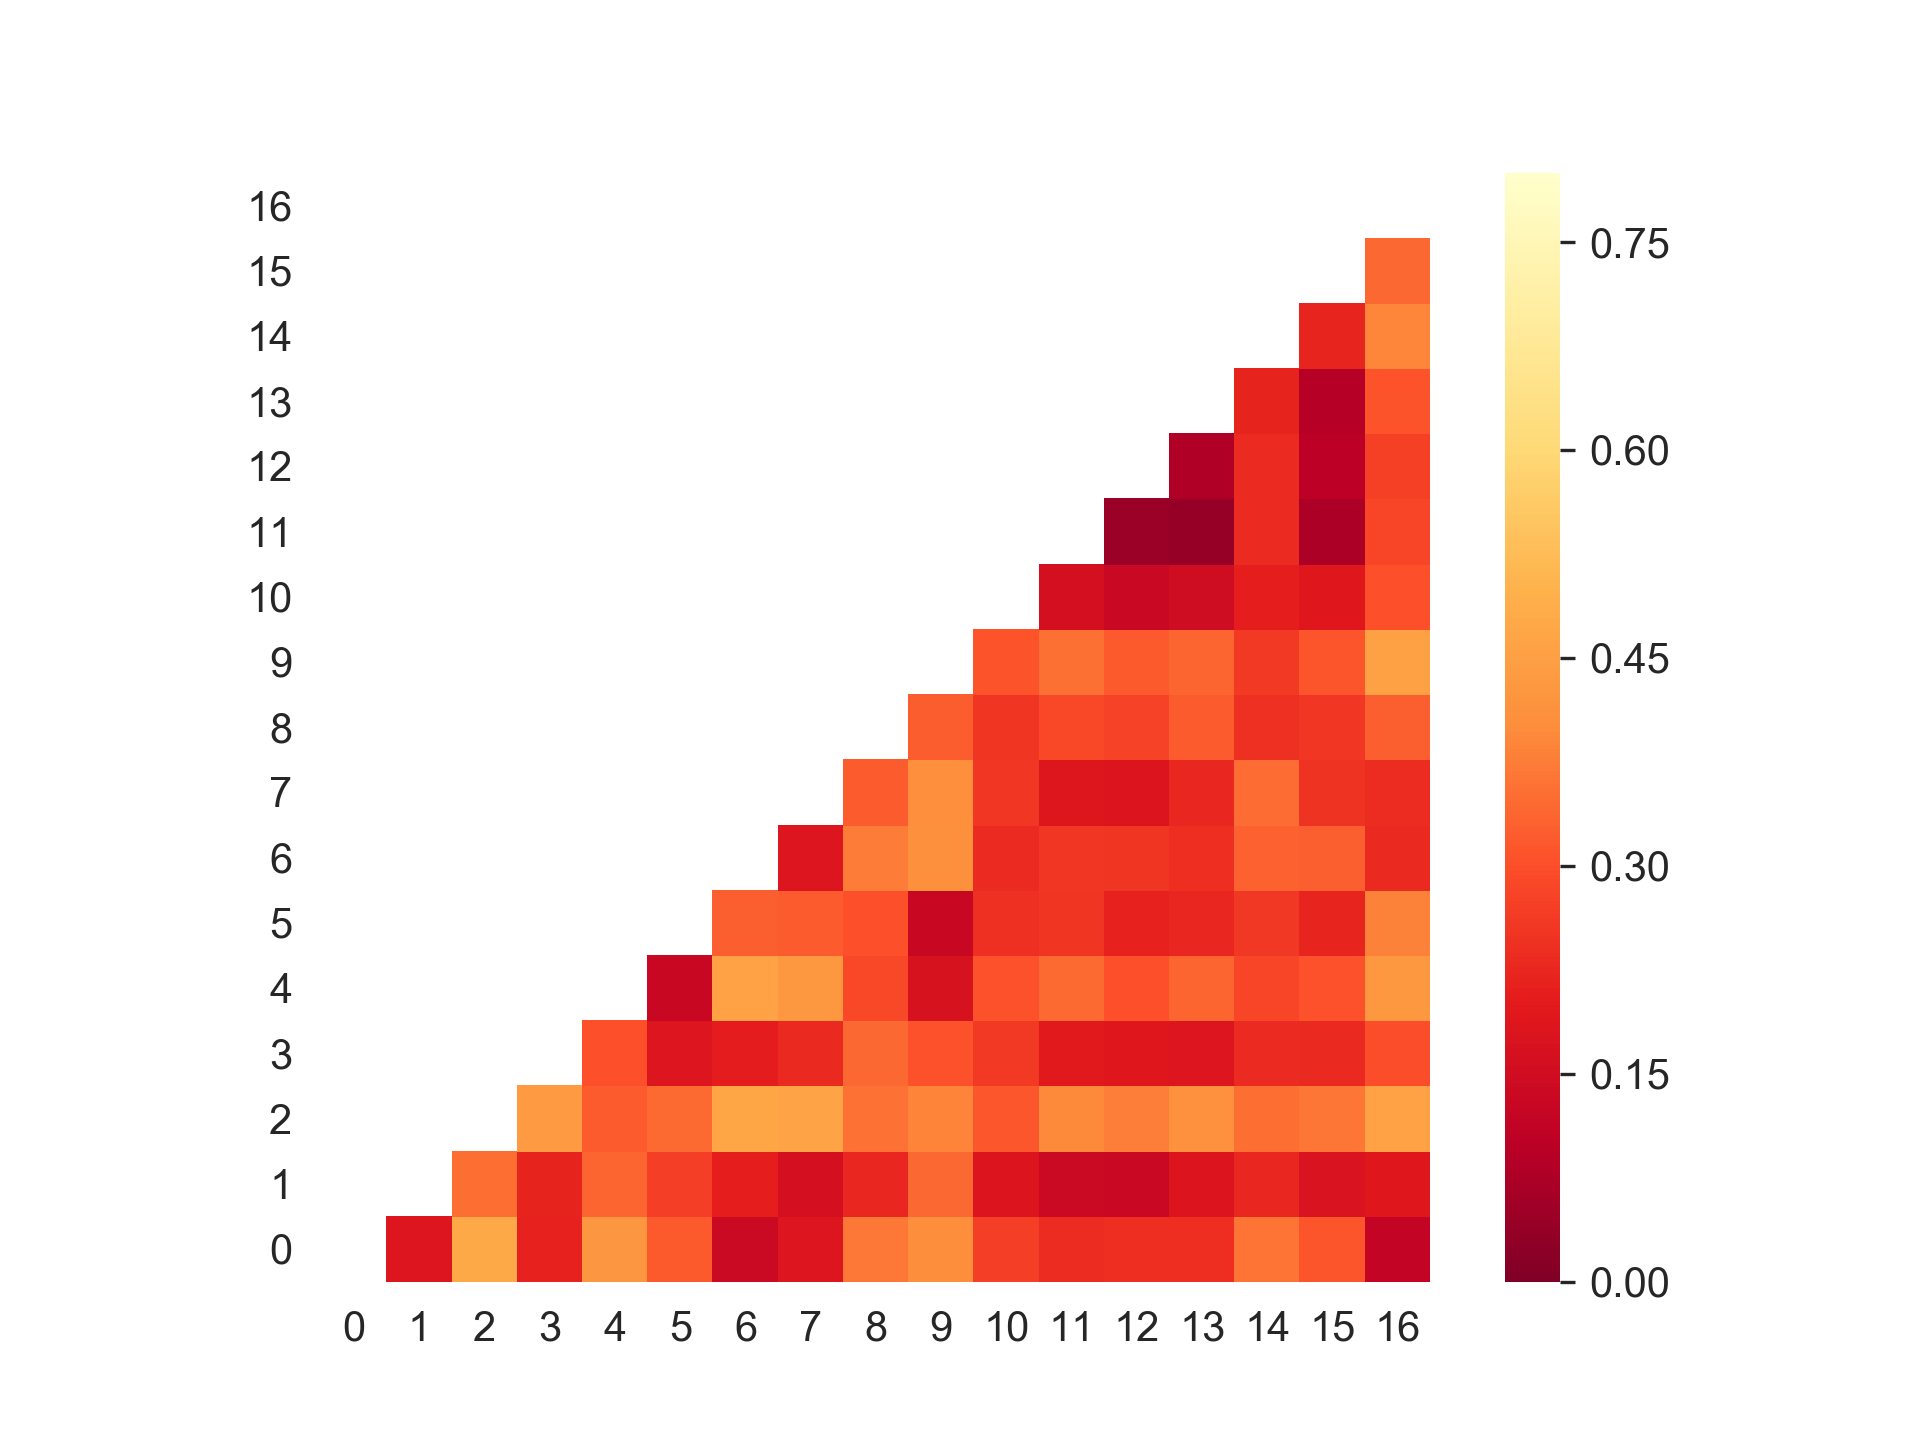
\includegraphics[width=0.5\textwidth]{bert_before_cleansing.png}\label{fig:bert_before_cleansing}}
  \hfill
  \subfloat[After cleansing.]{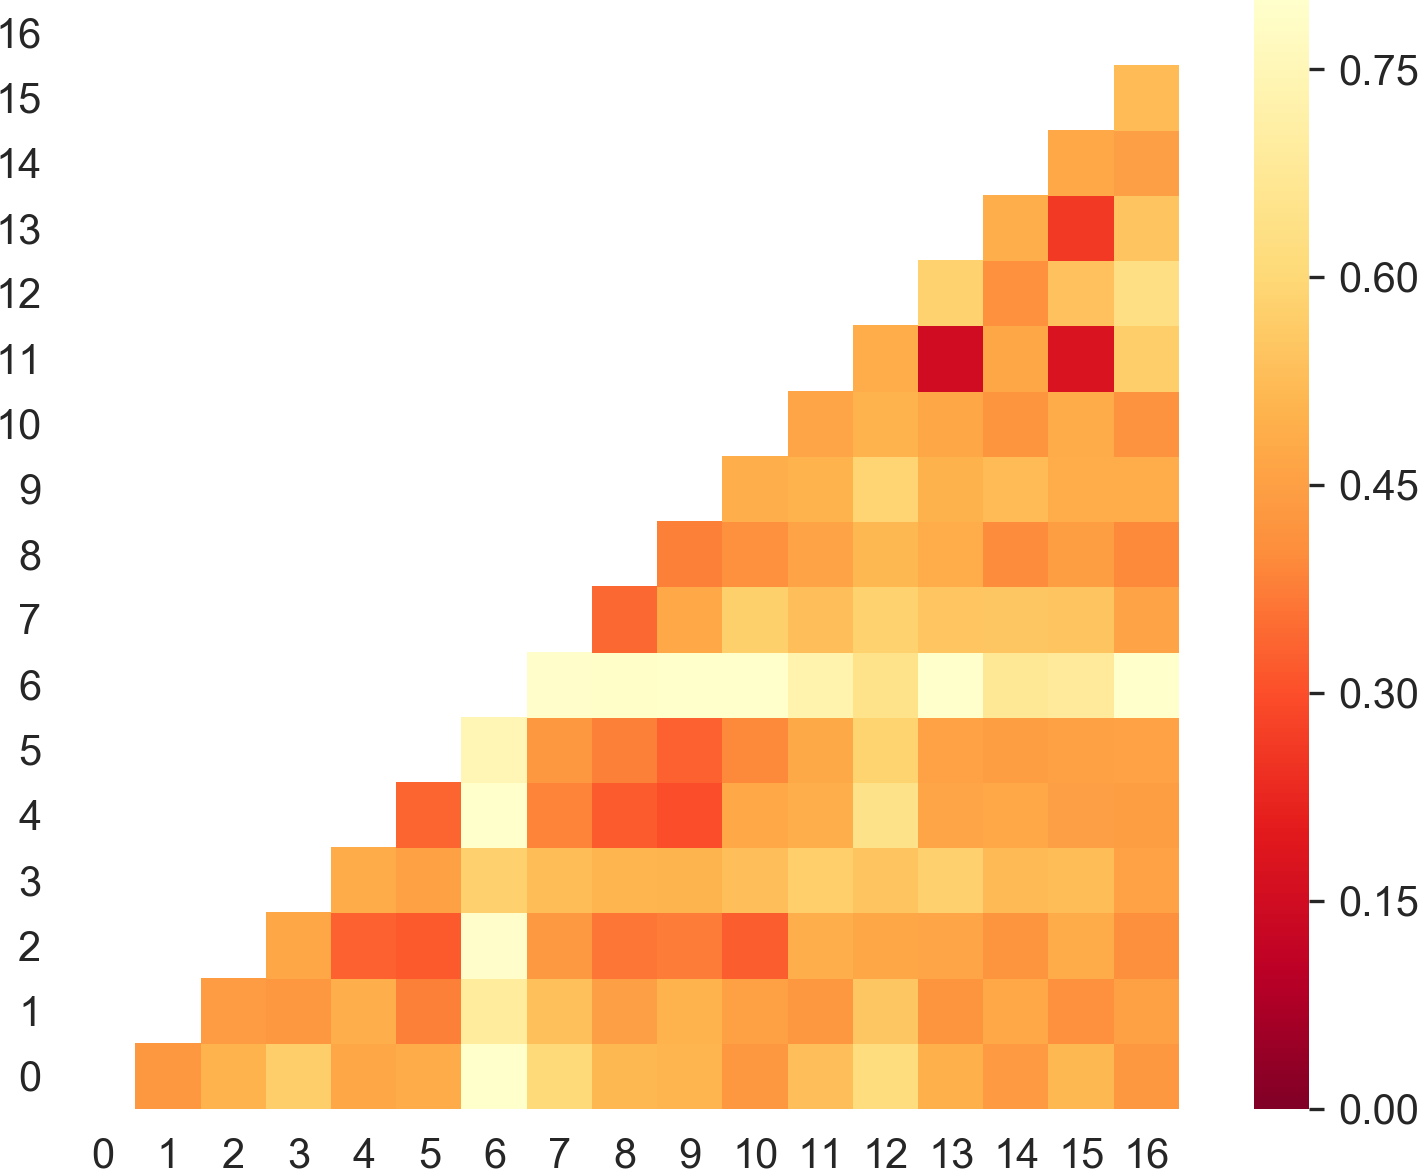
\includegraphics[width=0.5\textwidth]{bert_after_cleansing.png}\label{fig:bert_after_cleansing}}
  \caption{Bert pairwise template cosine distance.}
\end{figure}

\begin{figure}[!tbp]
  \centering
  \subfloat[Before cleansing.]{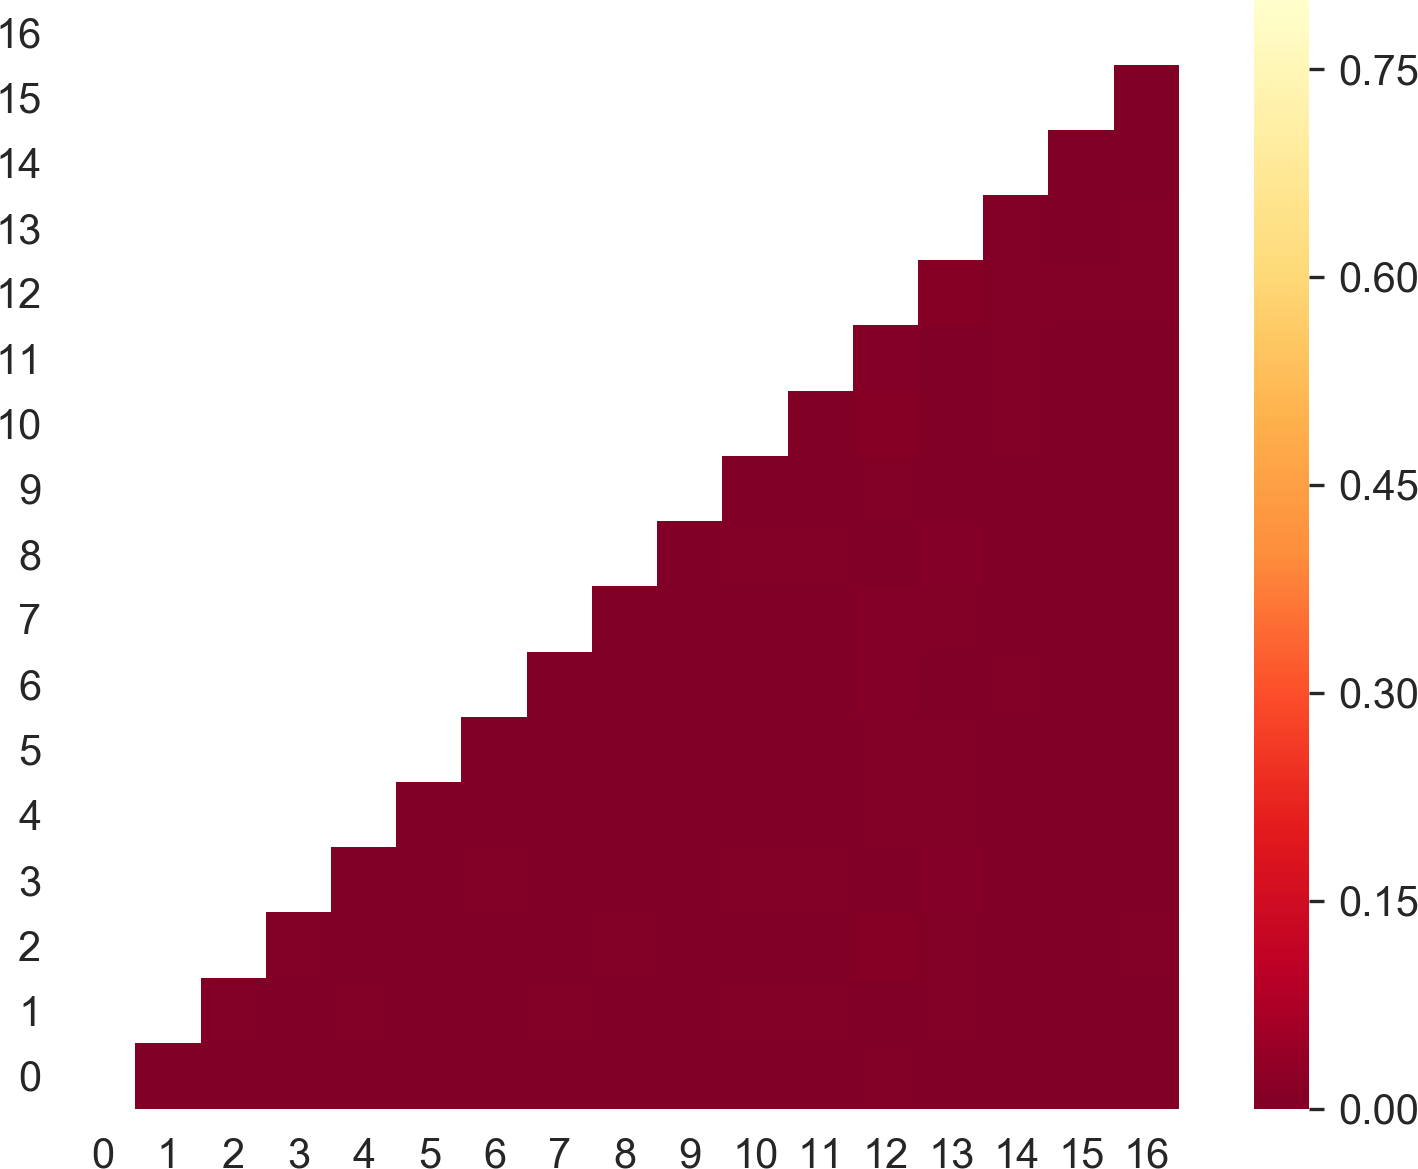
\includegraphics[width=0.5\textwidth]{gpt_before_cleansing.png}\label{fig:gpt_before_cleansing}}
  \hfill
  \subfloat[After cleansing.]{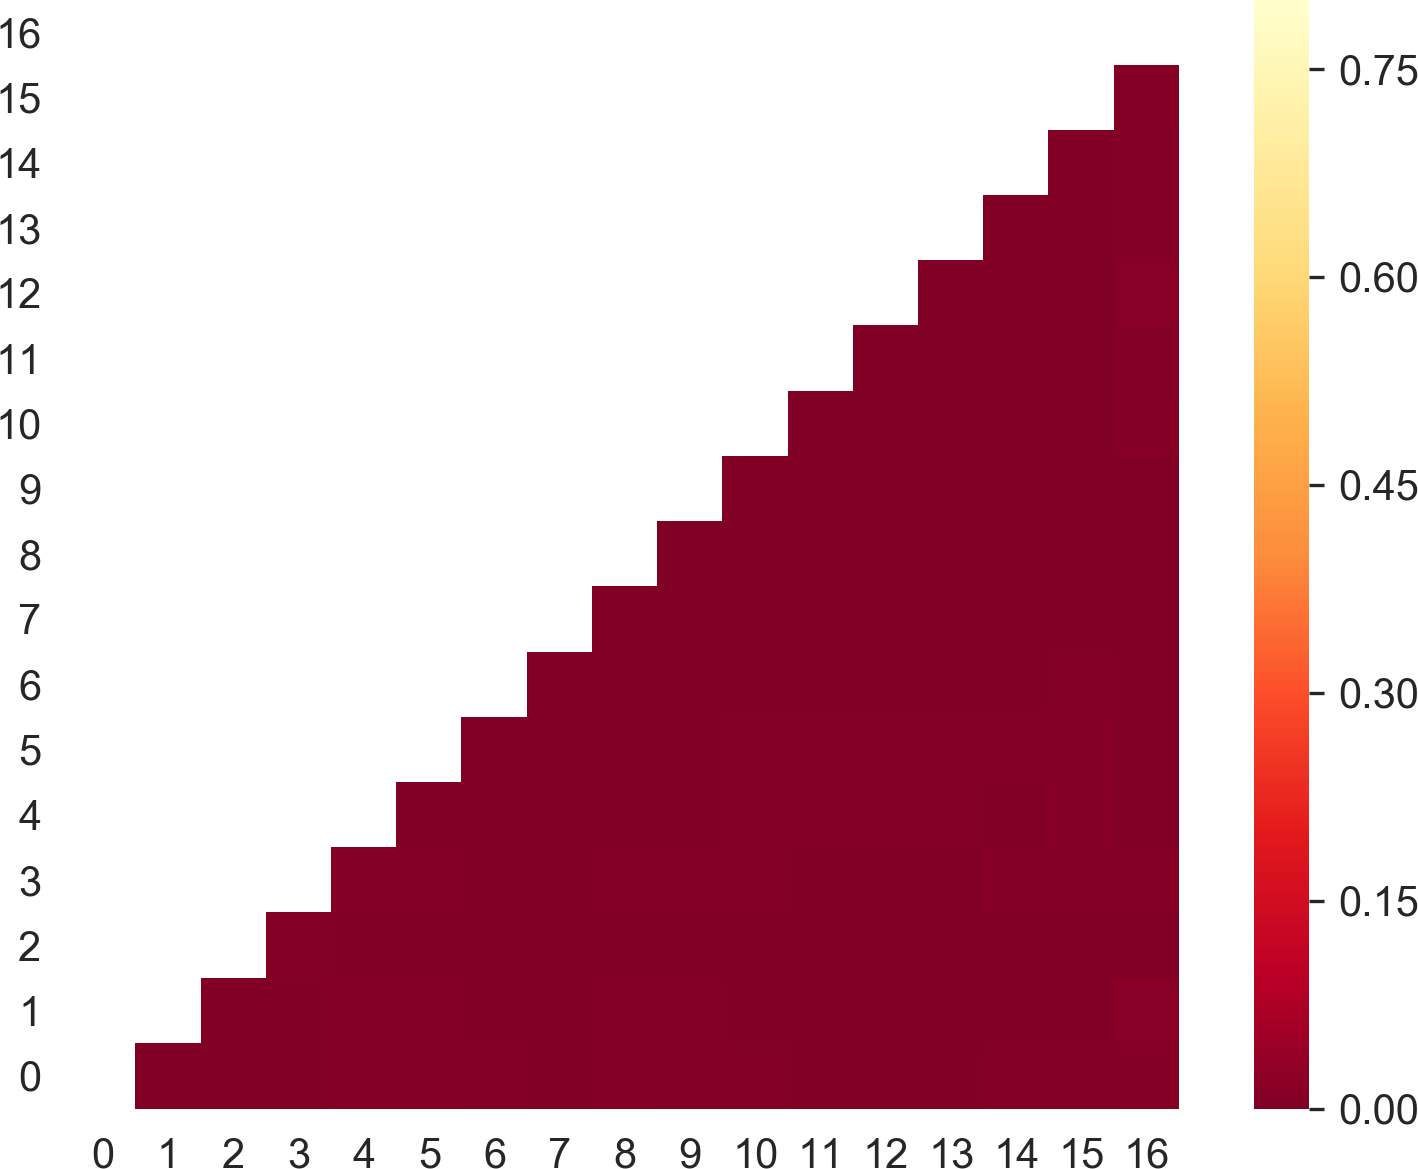
\includegraphics[width=0.5\textwidth]{gpt_after_cleansing.png}\label{fig:gpt_after_cleansing}}
  \caption{GPT-2 pairwise template cosine distance.}
\end{figure}

\begin{figure}[!tbp]
  \centering
  \subfloat[Before cleansing.]{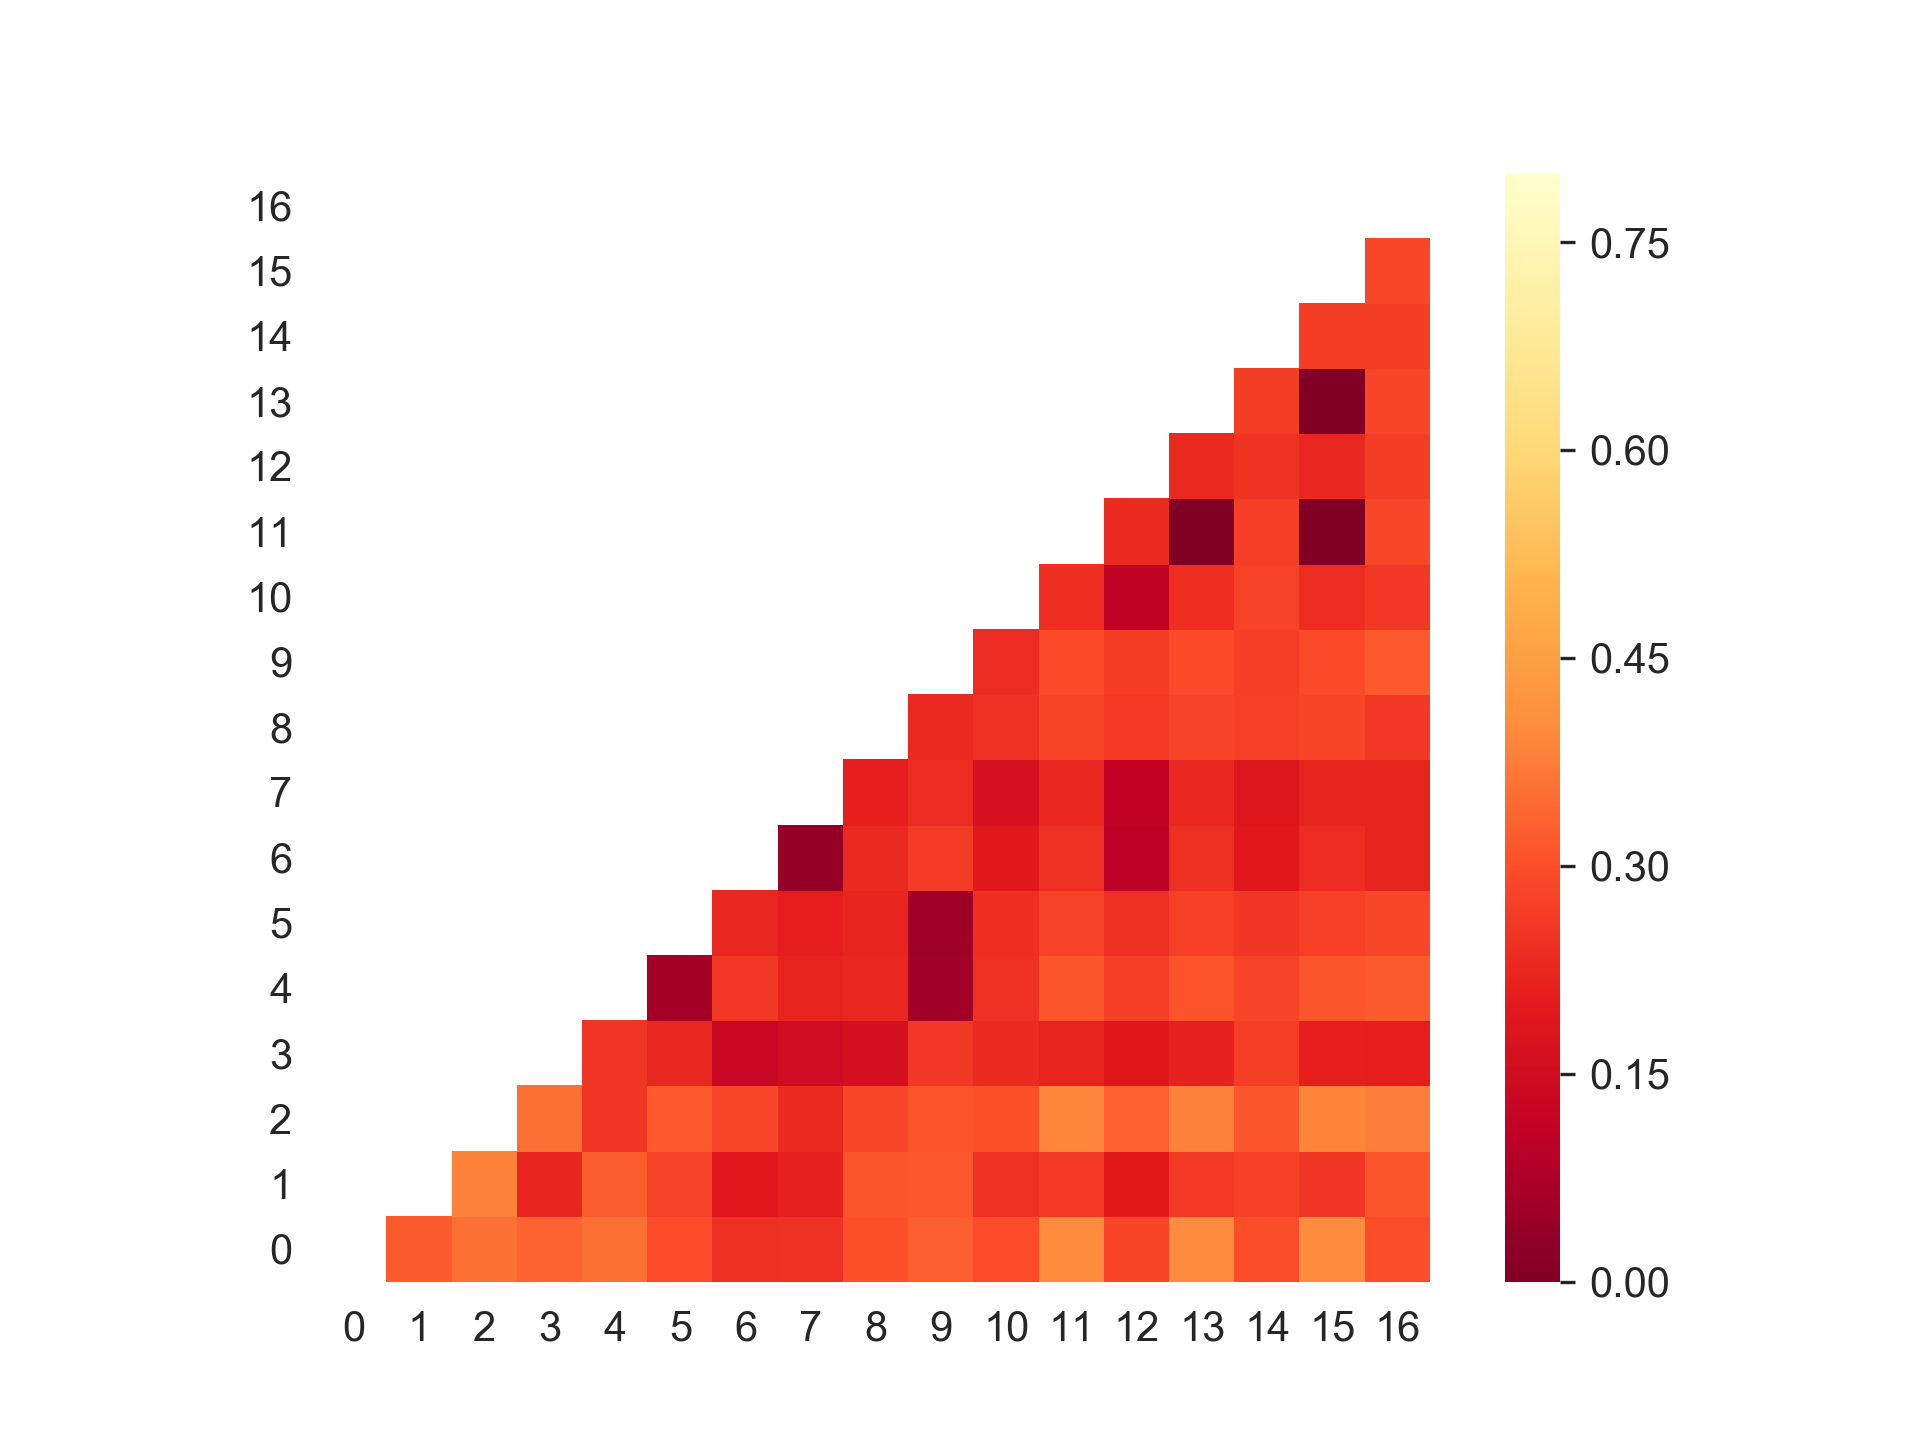
\includegraphics[width=0.5\textwidth]{xl_before_cleansing.png}\label{fig:xl_before_cleansing}}
  \hfill
  \subfloat[After cleansing.]{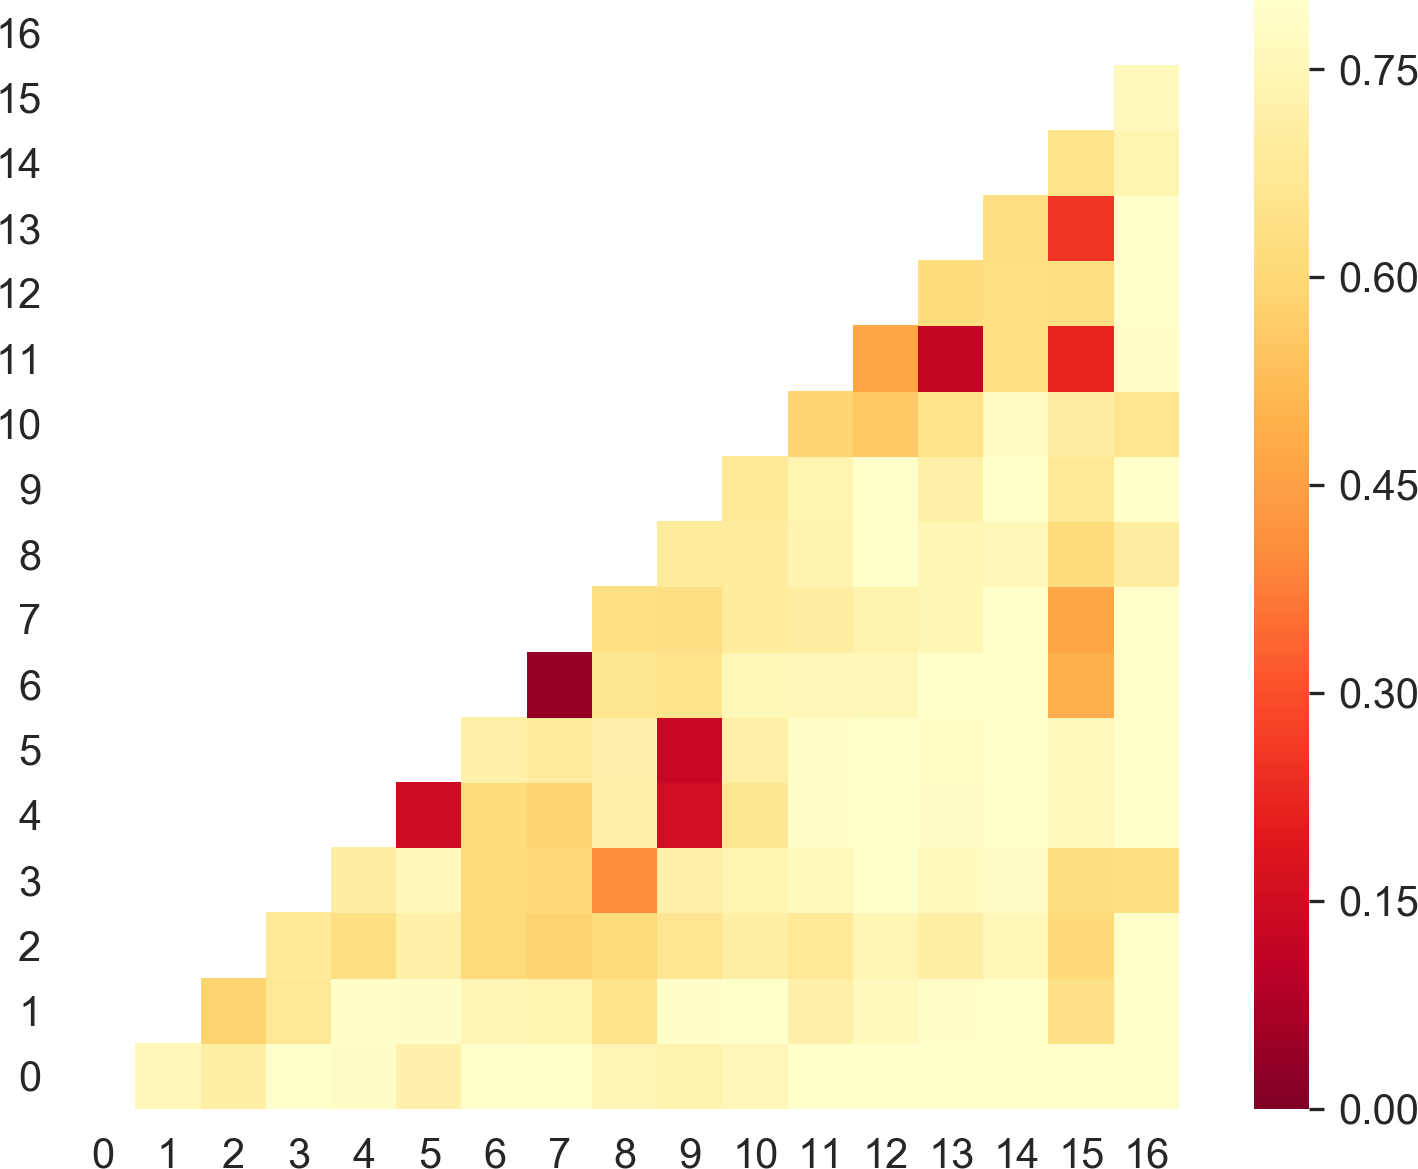
\includegraphics[width=0.5\textwidth]{xl_after_cleansing.png}\label{fig:xl_after_cleansing}}
  \caption{XL-Transformers pairwise template cosine distance.}
\end{figure}




\begin{table}[ht]
\begin{small}
\centering
\begin{tabular}{ c l } 
\toprule
Index & Template \\
\midrule
0 & $\langle*\rangle$ Creating image\\
1 & $\langle*\rangle$ VM $\langle*\rangle$ (Lifecycle Event)\\
2 & $\langle*\rangle$ During sync\_power\_state the instance has a pending task (spawning). Skip.\\
3 & $\langle*\rangle$ Instance $\langle*\rangle$ successfully.\\
4 & $\langle*\rangle$ Took $\langle*\rangle$.$\langle*\rangle$ seconds to $\langle*\rangle$ the instance on the hypervisor.\\
5 & $\langle*\rangle$ Took $\langle*\rangle$.$\langle*\rangle$ seconds to build instance.\\
6 & $\langle*\rangle$ Terminating instance\\
7 & $\langle*\rangle$ Deleting instance files $\langle*\rangle$\\
8 & $\langle*\rangle$ Deletion of $\langle*\rangle$ complete\\
9 & $\langle*\rangle$ Took $\langle*\rangle$.$\langle*\rangle$ seconds to deallocate network for instance.\\
10 & $\langle*\rangle$ Attempting claim: memory $\langle*\rangle$ MB, disk $\langle*\rangle$ GB, vcpus $\langle*\rangle$ CPU\\
11 & $\langle*\rangle$ Total memory: $\langle*\rangle$ MB, used: $\langle*\rangle$.$\langle*\rangle$ MB\\
12 & $\langle*\rangle$ memory limit: $\langle*\rangle$.$\langle*\rangle$ MB, free: $\langle*\rangle$.$\langle*\rangle$ MB\\
13 & $\langle*\rangle$ Total disk: $\langle*\rangle$ GB, used: $\langle*\rangle$.$\langle*\rangle$ GB\\
14 & $\langle*\rangle$ $\langle*\rangle$ limit not specified, defaulting to unlimited\\
15 & $\langle*\rangle$ Total vcpu: $\langle*\rangle$ VCPU, used: $\langle*\rangle$.$\langle*\rangle$ VCPU\\
16 & $\langle*\rangle$ Claim successful\\
\bottomrule
\end{tabular}
\caption{Templates before cleansing}
\label{tab:templates_before_cleansing}
\end{small}
\end{table}



\begin{table}[ht]
\begin{small}
\centering
\begin{tabular}{ c l } 
\toprule
Index & Template \\
\midrule
0 & Creating image\\
1 & VM  Lifecycle Event\\
2 & During sync power state the instance has a pending task spawning Skip\\
3 & Instance  successfully\\
4 & Took  seconds to  the instance on the hypervisor\\
5 & Took  seconds to build instance\\
6 & Terminating instance\\
7 & Deleting instance files\\
8 & Deletion of complete\\
9 & Took  seconds to deallocate network for instance\\
10 & Attempting claim memory  MB disk  GB vcpus  CPU\\
11 & Total memory  MB used  MB\\
12 & memory limit  MB free  MB\\
13 & Total disk  GB used  GB\\
14 & limit not specified defaulting to unlimited\\
15 & Total vcpu  VCPU used  VCPU\\
16 & Claim successful\\
\bottomrule
\end{tabular}
\caption{Templates after cleansing}
\label{tab:templates_after_cleansing}
\end{small}
\end{table}

\subsection{Finetuning}
As described in \ref{sec:finetuning}, finetuning can potentially help to produce word embeddings that are more adequate for solving a certain task, it is thus desirable to produce word embeddings that help solving the task of anomaly detection better. As described in \ref{sec:word_vectorization}, a high cosine distance between semantically different templates is required. The dataset that consists of the templates in table \ref{tab:templates_after_cleansing} has been chosen for finetuning. Since the pre-trained language models at hand (namely \textit{bert-base-uncased} and \textit{gpt2}) have been trained on a large corpus, finetuning would also need to be executed on a sufficiently large corpus. Since this is not the case, the results of finetuning for a maximum of four epochs, as suggested by the Bert authors \cite{devlin2018bert}, does not yield the desired results. As it can be seen in figure \ref{fig:cos_distance_finetuning}, it was not possible to increase the cosine distances between templates on the task of Masked LM (as described in \ref{Bert}), compared to the cosine distances depicted in figure \ref{fig:bert_after_cleansing}. The average distance between templates dropped to 0.3016 from 0.4449. The fact that the loss on the evaluation part of the dataset is not decreasing adequately, as shown in figure \ref{fig:finetuning_loss}, shows that training on such a small corpus is not able to generalise well enough, which makes finetuning on the default learning task not useful in this case. Since the Huggingface Transformers library does not offer out of the box finetuning interfaces for GPT-2 and XL-Transformers on the same task as for Bert, they are not further investigated for finetuning.

\begin{figure}[H]
  \centering
  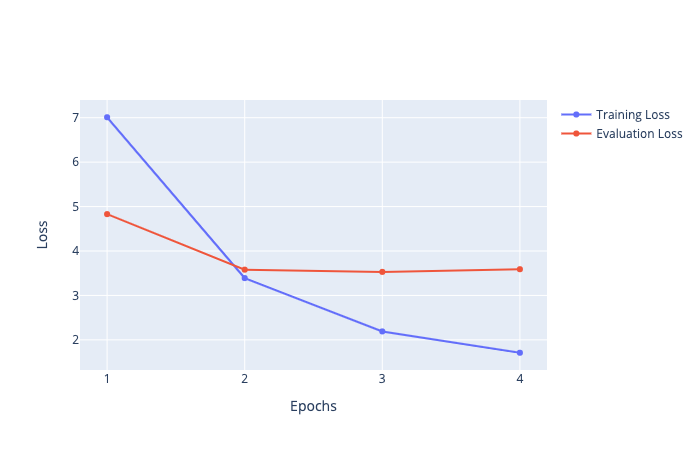
\includegraphics[width=12cm,height=8.5cm]{finetuning_loss.png}\\
  \caption{Training and evaluation loss for finetuning on masked LM.}
  \label{fig:finetuning_loss}
\end{figure}

\begin{figure}[h]
  \centering
  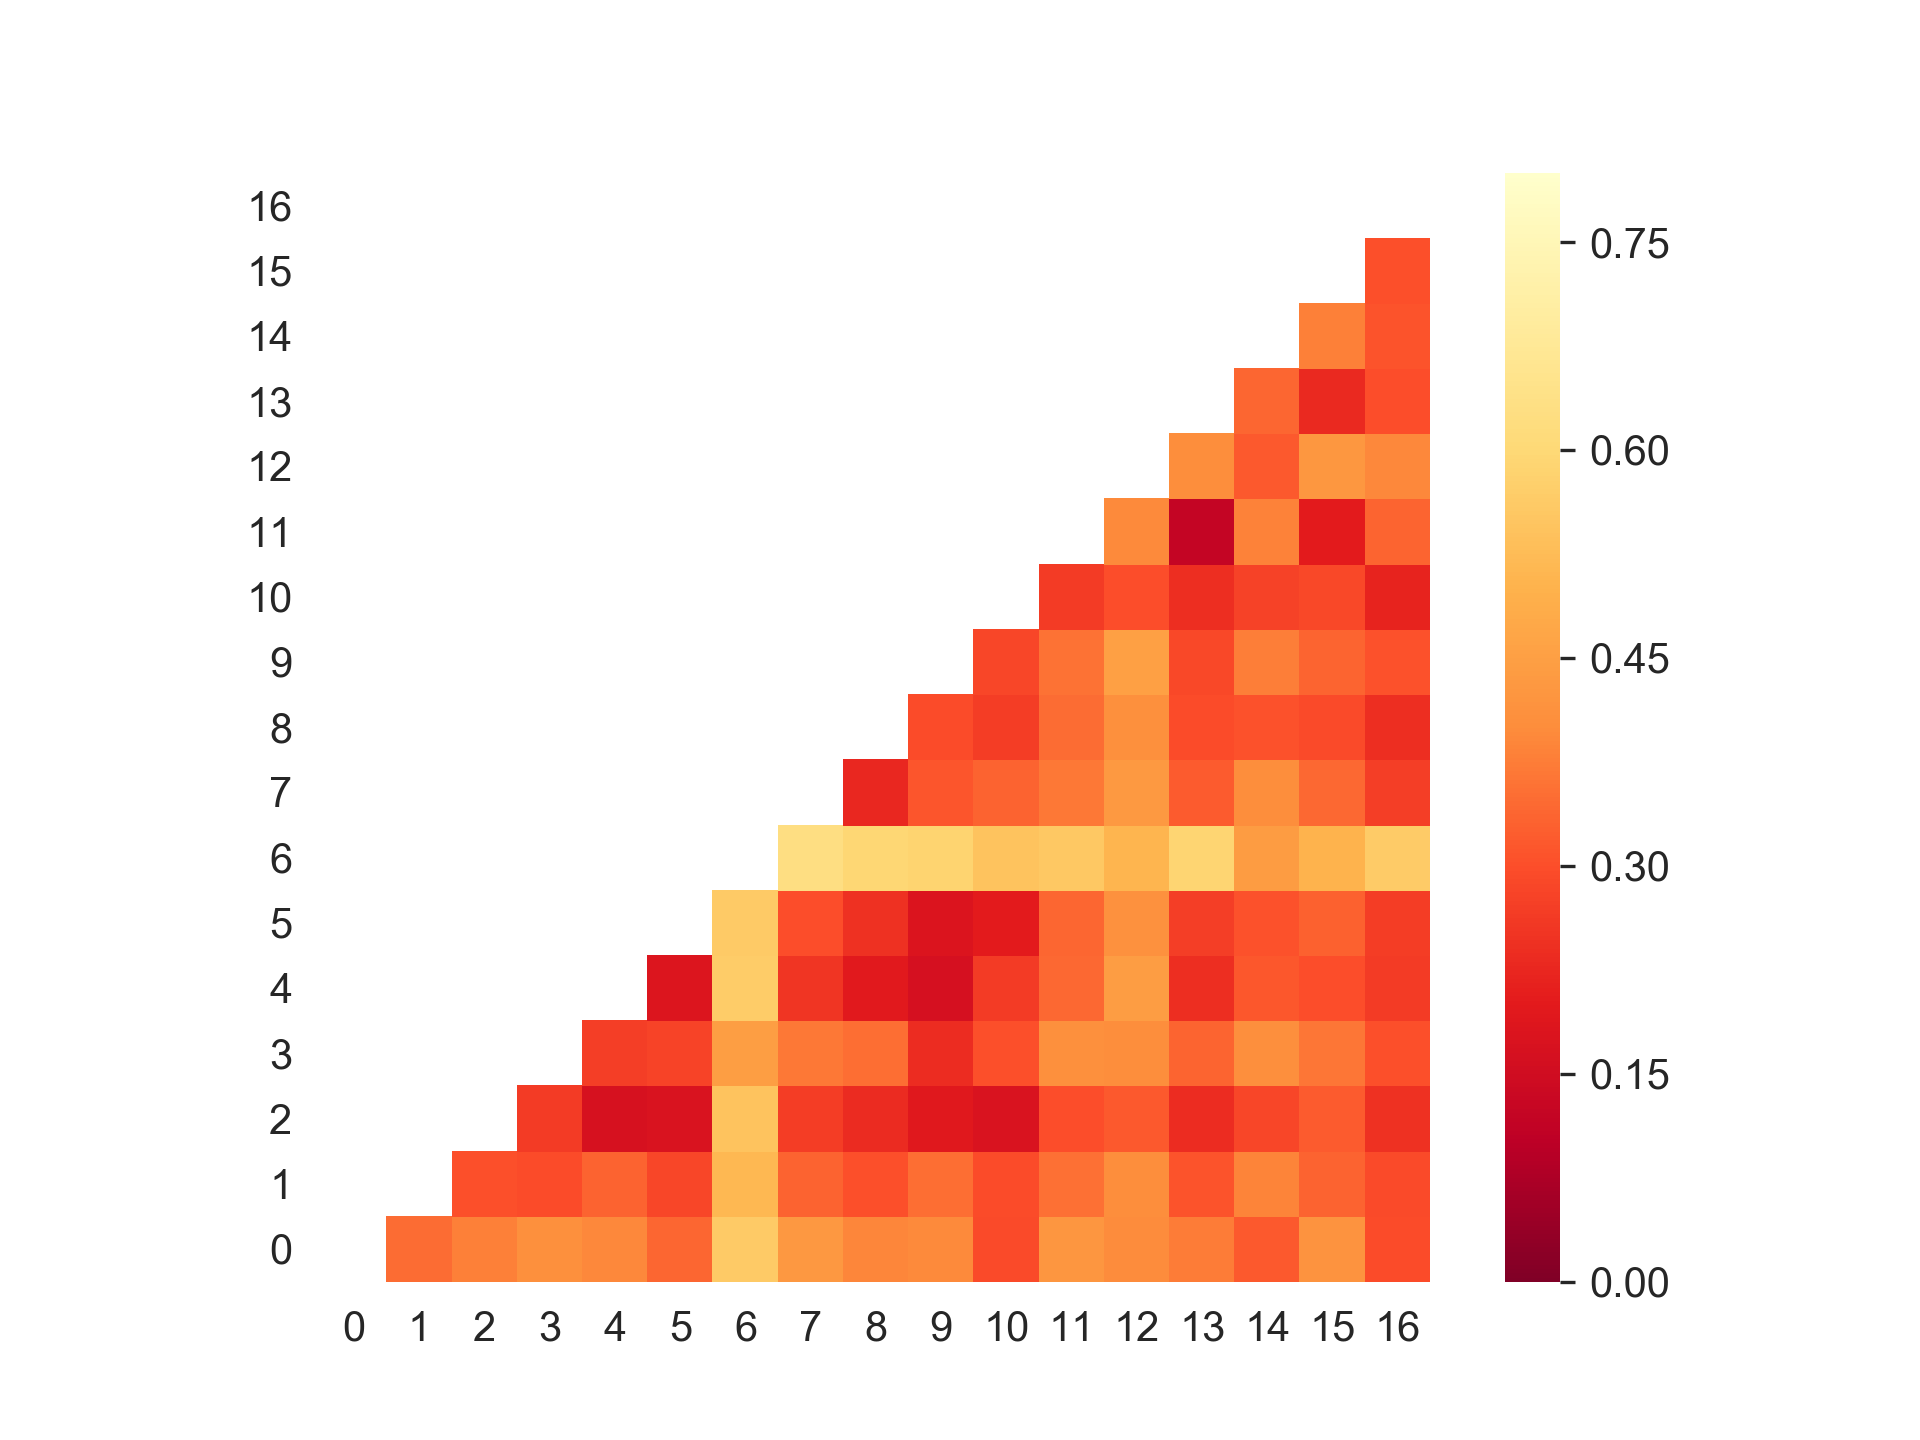
\includegraphics[width=12cm,height=10cm]{bert_finetuning_cleansed.png}\\
  \caption{Cosine distance between templates after cleansing and finetuning}
  \label{fig:cos_distance_finetuning}
\end{figure}


\subsection{Hyperparameters}
In order to find well-suited parameters for the LSTM model, it was first applied to the problem using a minimal configuration. With the help of a grid-search, running simulations with different configurations, the following hyperparameters have proven to yield the most satisfying results:
\begin{itemize}
	\item 512 hidden units for the bidirectional LSTM, with one layer
	\item two fully connected layers with 512 units $\rightarrow$ 256 units $\rightarrow$ output size
	\item dropout of 0.1 between every layer
	\item input sequence length of 7
	\item 60 Epochs of training
\end{itemize}



\subsection{Classification \label{sec:results-classification}}

\subsection{Regression \label{sec:results-regression}}

\section{Discussion of Results}
%TODO box plots of loss values in 